\section{Risultati Ottenuti}
I risultati, che verranno dettagliatamente mostrati nelle sezioni successive, possono essere riassunti generalmente
come dei risultati positivi, sia in fatto di performance che di policy applicate. Specificatamente 
al tempo e' possibile mostrare come il tempo generale della simulazione dipenda principalmente dall'applicazione
del controllore e quindi dal calcolo della Neural ODE e tutte le operazioni che ne conseguono. 

\begin{tabular}{ |p{2,57cm}||p{2,57cm}|p{2,57cm}|p{2,57cm}|p{2,57cm}|  }
	\hline
	\multicolumn{5}{|c|}{Tempo Impiegato (HH:MM:SS)} \\
	\hline
	Tipologia di Test & Nessun Intervento & Intervento Non Farmaceutico & Intervento Farmaceutico & Intervento Farmaceutico e Non\\
	\hline
	Singlerun (50 PdI) & 0:00:14 & 0:09:08 & 0:00:13 & 0:02:54\\
	Ensemblerun (5 ripetizioni, 50 PdI) & 0:00:34 & 00:41:07 & 0:00:26 & 0:54:21\\
	\hline
\end{tabular}

\begin{tabular}{ |p{2,57cm}||p{2,57cm}|p{2,57cm}|p{2,57cm}|p{2,57cm}|  }
	\hline
	\multicolumn{5}{|c|}{Tempo Impiegato (HH:MM:SS)} \\
	\hline
	Tipologia di Test & Nodi Infetti Iniziali Variabili & Valore di Migrazione Variabile & Nodi della Rete Variabile & Copertura dei Nodi Variabile\\
	\hline
	Paramscan & 0:00:13 & 0:00:33 & 0:00:33 & 0:00:13\\
	\hline
\end{tabular}

Queste lunghe tempistiche derivano dal calcolo delle contromisure non farmaceutiche applicabili alla popolazione, 
e per questo, le contromisure farmaceutiche, se applicate con il giusto tempismo, oltre a dare un notevole 
apporto alla riduzione della diffusione della pandemia \ref{fig:comparison_vax_1} \ref{fig:comparison_vax_2}
\ref{fig:comparison_vax_3} \ref{fig:comparison_vax_4}, permettono una notevole riduzione dei tempi computazionali.
\newpage

\subsection{Nessun intervento}
Il seguente grafico \ref{fig:abm_no_intervent} mostra l'andamento delle curve del modello
quando questo viene eseguito senza alcuna tipologia di intervento. Questo andamento è mostrato 
in maniera cumulativa rispetto all'andamento dei singoli agenti, i quali possono mostrare comportamenti 
differenti tra loro.

\begin{minipage}{\linewidth}
	\centering
	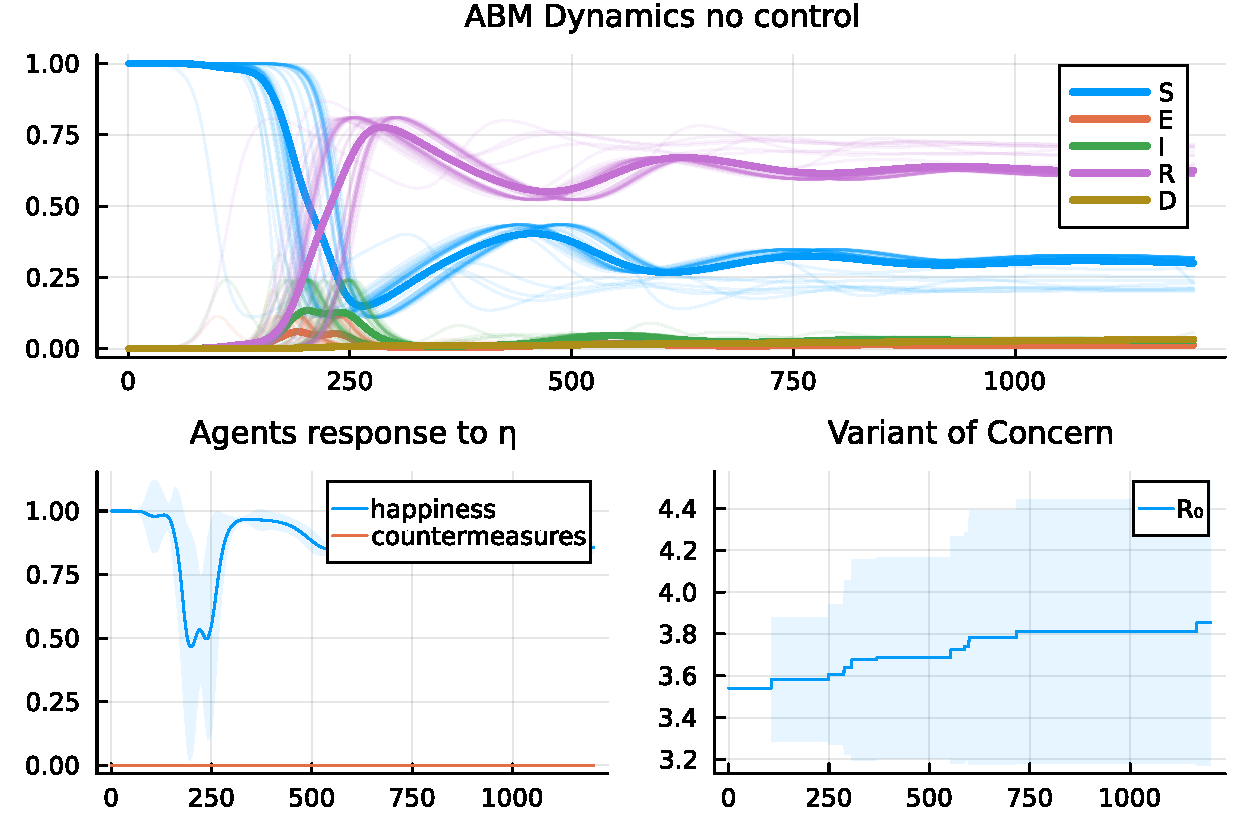
\includegraphics[width=\textwidth]{img/SocialNetworkABM_NO_CONTROL.pdf}
	\captionof{figure}{Grafico cumulativo del modello senza senza alcun tipo di intervento}
	\label{fig:abm_no_intervent}
\end{minipage}

Complessivamente l'andamento del modello è similare all'andamento standard di un modello di tipo  
SEIR, con qualche variazione dipendente dai fattori di stocasticità intrisechi del modello; che in questo
caso non sono troppo presenti. Il grafico mostra le traiettorie più comuni delle curve cumulate del modello, 
dove vengono messe in evidenza i percorsi più utilizzati. 

Come è possibile notare, il numero di individui suscettibili crolla drasticamente
per via della diffusione rapida e simil esponenziale che ha il virus. Questa viene emulata
dall'altrettanto rapida crescita di individui guariti (recovered) che però, per via
di come è stato definita la condizione di guariti, non sono immuni alle varianti del virus, permettendo 
di modellare una possibile ciclicità dell'epidemia data dalla perdita di immunità della popolazione. 
Queste proprietà contribuiscono ad un andamento ciclico delle curve. Si può notare come 
la curva associata all'andamento degli individui nella classe \emph{D} abbia una crescita lineare, 
seppur non troppo evidente.

A seguire si può osservare come la curva associata alla variabile di happiness del modello,
valore che serve per bilanciare la durezza delle misure di controllo per evitare 
di cadere in un ciclo funzionale ma insostenibile, mostra un comportamento alquanto bizzarro.
Questo è dovuto principalmente a come viene definita la funzione di controllo della felicità \ref{fig:happinessf}.
Si osserva inoltre che la curva tende ad un \emph{plateau} passato il periodo della "prima ondata".

Questo comportamento principalmente irrealistico e associato alla definizione che è stato fatto della 
funzione \textbf{happiness} \ref{fig:happinessf}. Il comportamento di questa curva non è completamente 
realistico, ma è comunque utilizzabile per lo scopo di mantenere sotto controllo le contromisure $\eta$.

\begin{minipage}{\linewidth}
	\centering
	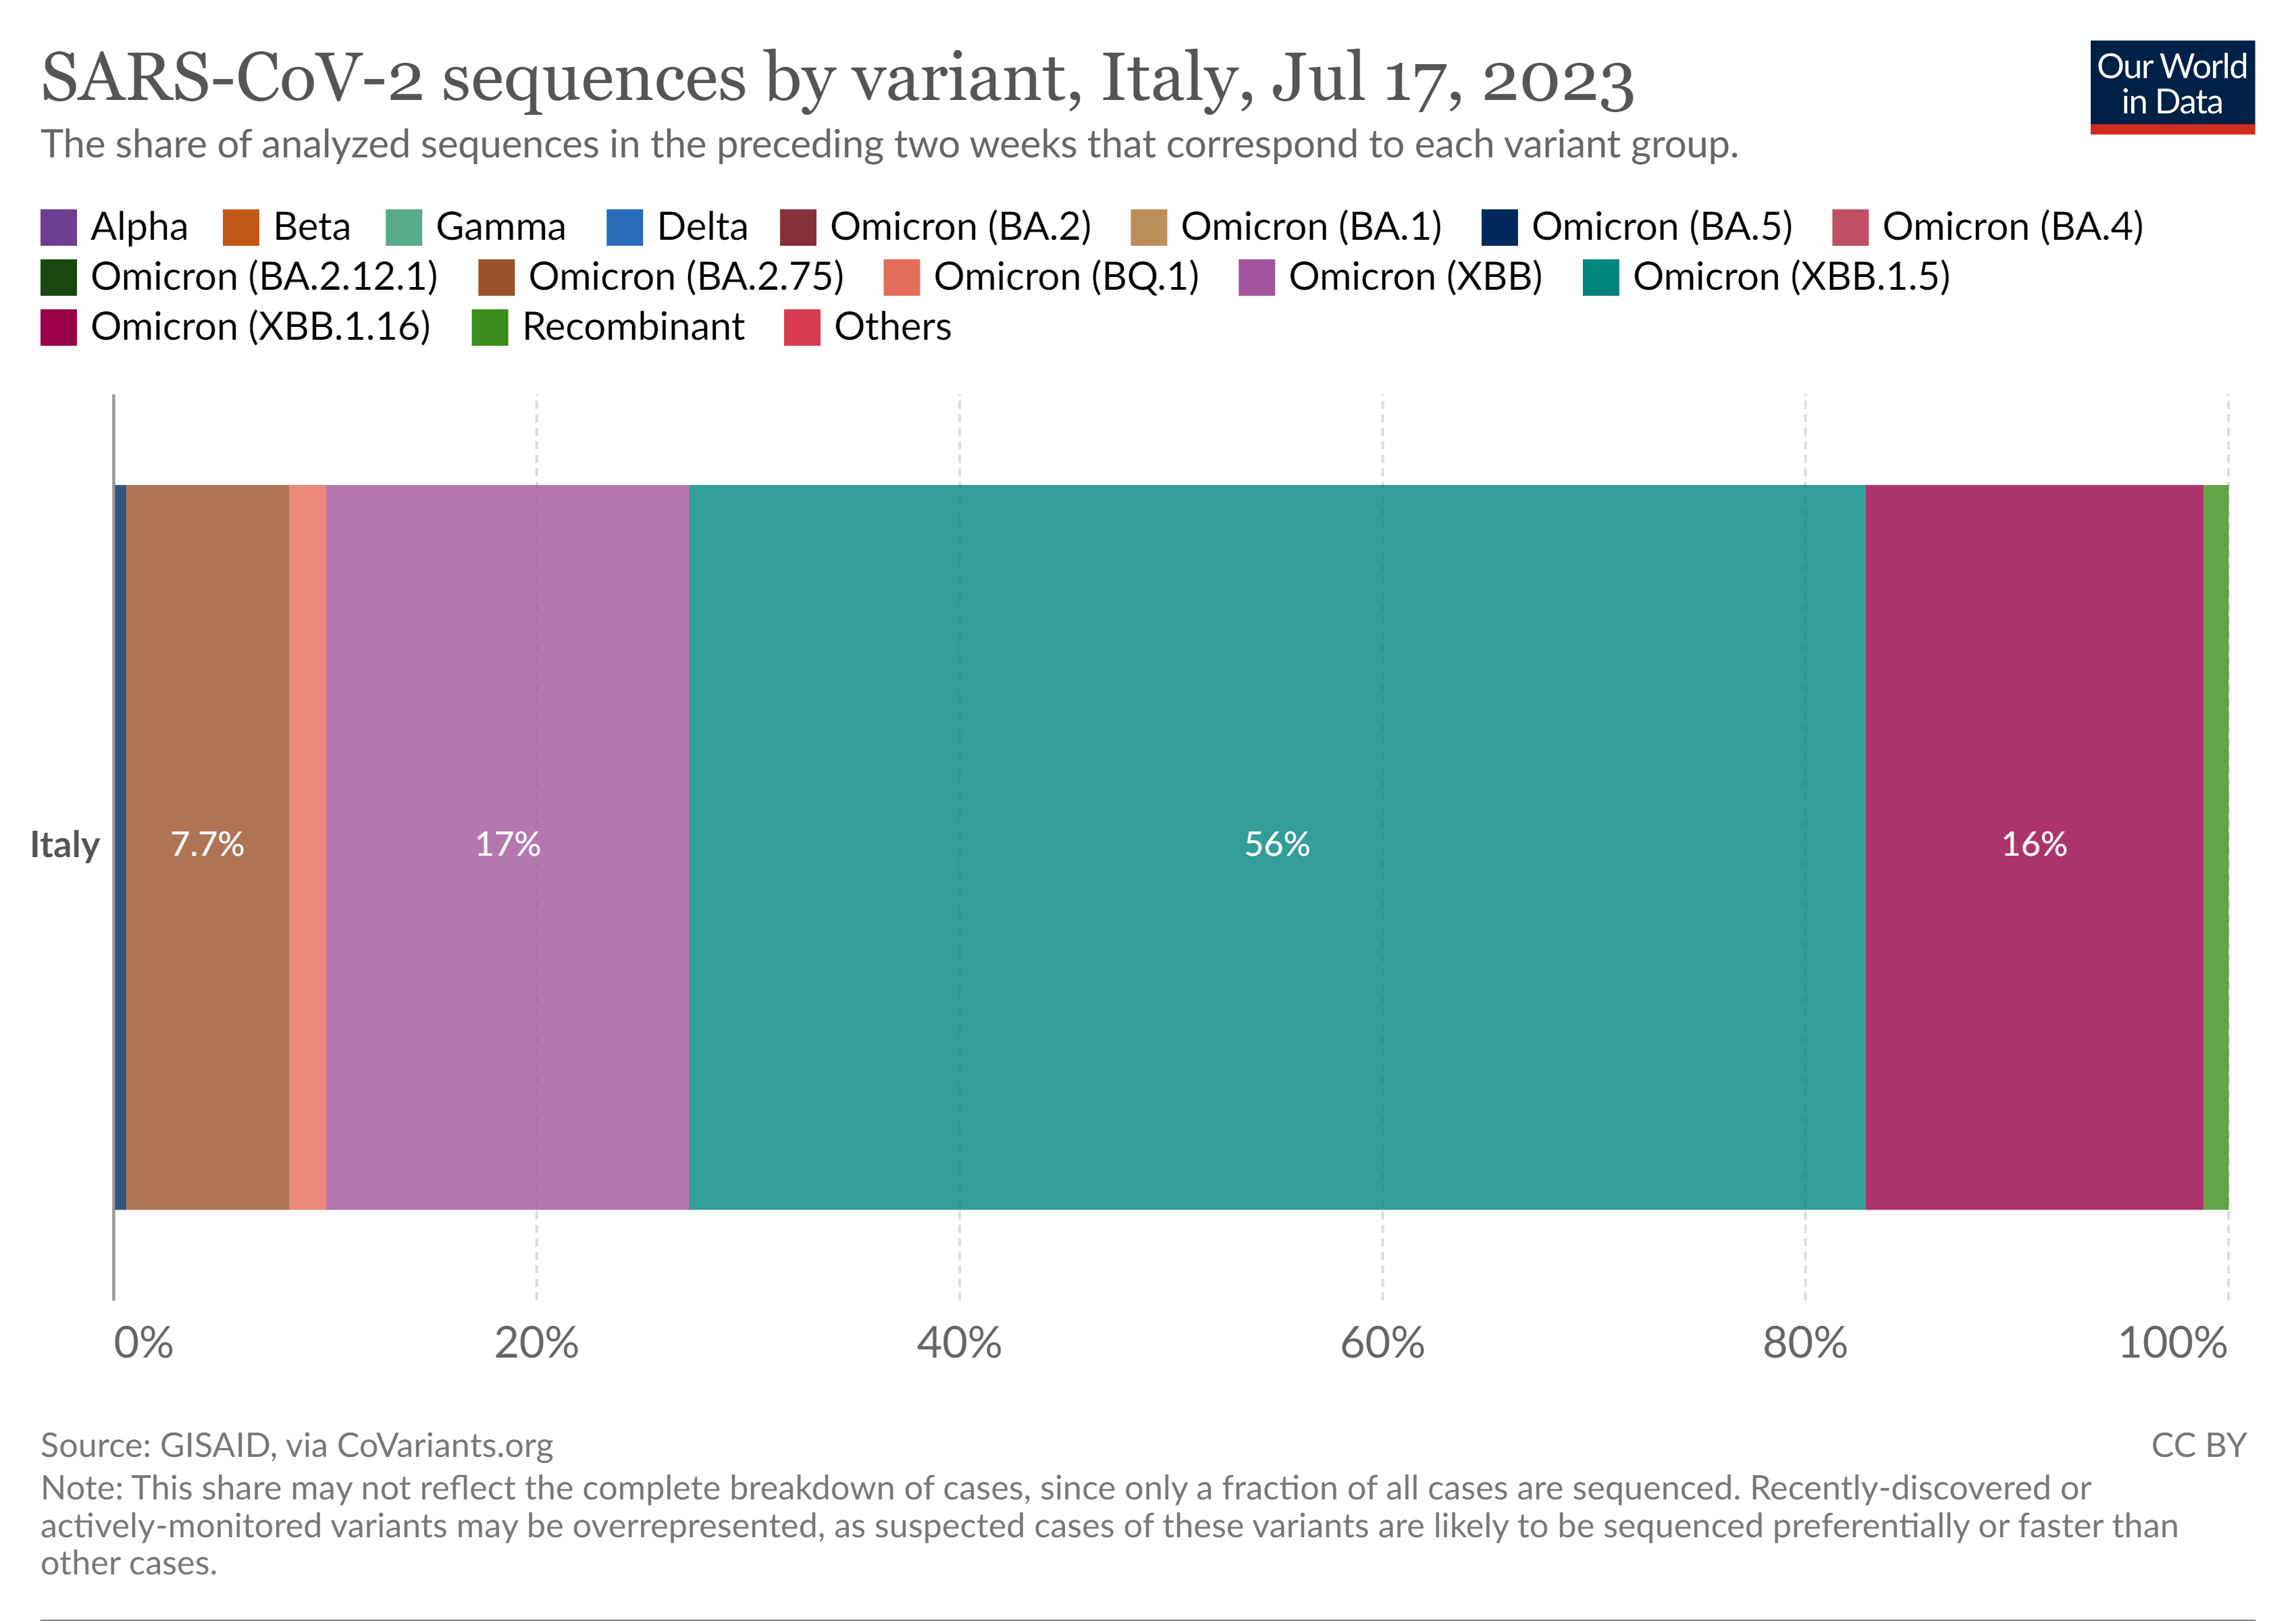
\includegraphics[width=\textwidth]{img/coronavirus-data-explorer.png}
	\captionof{figure}{Grafico delle mutazioni del virus SARS-COV2 preso da Our World in Data}
	\label{fig:covid_mutation}
\end{minipage}

Infine si nota come, seppur la definizione della funzione associata alla creazione di una
nuova \emph{VOC} \ref{fig:voc} sia semplicistica e irrealistica, il grafico mostra come 
su un periodo di circa 3 anni, associabile alla durata del periodo covid, 
il numero di VOC sia pressochè sovrapponibile con quanto osservato dai dati 
raccolti durante la pandemia \ref{fig:covid_mutation}. 
\newpage

\subsection{Intervento non farmaceutico}
Il seguente grafico \ref{fig:abm_intervent} mostra l'andamento delle curve del modello
quando questo viene eseguito tramite l'applicazione di una qualche tipologia di intervento non farmaceutico. 
Le contromisure sono rappresentate come un insieme di valori appartenenti all'intervallo $[0, 1)$ 
le quali rappresentano cumulativamente un insieme di metriche differenti non esplicite che vanno a definire 
un insieme di misure di controllo. Le misure di controllo cercano di mimicare quelle associate al progetto 
\textbf{OxCGRT} \cite{Hale2021} il quale ha lo scopo di misurare la durezza delle contomisure applicate in un determinato paese; 
questo valore è composito di 9 metriche: \emph{chiusura delle scuole; chiusura dei luoghi di lavoro; 
cancellazione di eventi pubblici; restrizioni agli assembramenti pubblici; 
chiusura dei trasporti pubblici; obbligo di rimanere a casa; campagne di informazione pubblica; 
restrizioni agli spostamenti interni e controlli sui viaggi internazionali}.

\begin{minipage}{\linewidth}
	\centering
	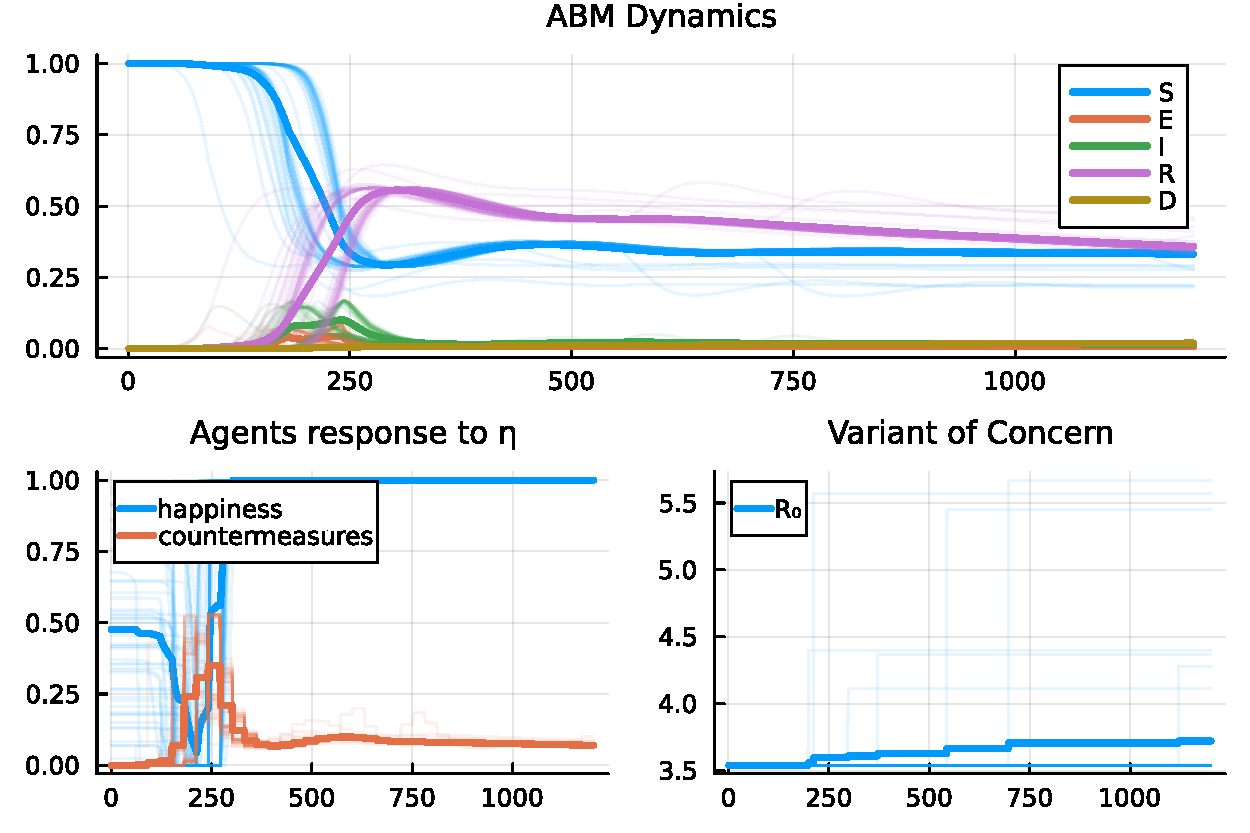
\includegraphics[width=\textwidth]{img/SocialNetworkABM_CONTROL.pdf}
	\captionof{figure}{Grafico cumulativo del modello con intervento non farmaceutico del controllore}
	\label{fig:abm_intervent}
\end{minipage}

Queste metriche sono metriche reali ma che nel modello vengono viste come un insieme unico, associabile 
ad una somma di medie dei valori di ogni metrica. Questa scelta porta a non avere un indice molto chiaro
ma permette comunque di avere un idea generale estremamente immediata dell'effetto che queste hanno sul modello.

Si nota come con l'applicazione di un insieme di contromisure, più o meno stringenti a seconda del periodo osservato, 
possiamo osservare come le curve epidemiologiche tendono ad appiattirsi, soprattutto quelle associate ai compartimenti 
\textbf{E, I}, le quali influenzano le curve \textbf{S, R}. In questo caso la ciclicità del modello viene meno. 

Altro dato interessante è il numero di VOC che è diminuito rispetto al modello senza intervento.
Questo dipende generalmente dal comportamento delle contromisure. Infatti queste quando vengono applicate, 
oltre a influenzare il parametro \textbf{happiness}, vanno ad influenzare anche la matrice di flusso \ref{fig:migration matrix}
andando a ridurne i valori presenti. Questo fa si che oltre a dilazionare la diffusione della pandemia, 
va a dilazionare il comportamento della funzione che si occupa di generare una VOC \ref{fig:voc}. 

Questa infatti può attivarse sse nel nodo sono presenti individui infetti, in quanto non è stata modellata la 
possibilità che spontaneamente una nuova variante arrivi in un nuovo nodo senza un veicolo umano. Perciò 
applicare delle contromisure permette anche a contenere la diffusione di VOC nella popolazione osservata.

Si può osservare come la variabile di controllo \textbf{happiness} segua molto attentamente l'andamento sia delle 
contromisure che della pandemia, arrivando all'inizio della pandemia quando le contromisure sono più stringenti 
a diventare pressoche nulla. Successivamente, pur mantenendo un livello di contromisure sostenuto, la media
del valore di controllo tende ad alzarsi, seguendo il valore del compartimento \textbf{R}. Questo approccio sembra 
imitare il generale andamento della risposta che la popolazione italiana ha avuto alle prime misure di contenimento 
applicate realmente durante la pandemia da COVID-19.
\newpage

\subsection{Intervento farmaceutico}
Il seguente grafico \ref{fig:abm_vaccine} mostra l'andamento delle curve del modello
quando questo viene eseguito tramite l'applicazione di una qualche tipologia di intervento farmaceutico.
Questo grafico dipende enormemente da quando viene trovato e successivamente applicato un intervento 
farmaceutico alla popolazione. Prima viene applicato un intervento farmaceutico più le curve si modificano 
e sono differenti dalll'andamento senza intervento \ref{fig:abm_no_intervent}, mentre più tempo passa più
il comportamento tende ad assomigliarsi.

\begin{minipage}{\linewidth}
	\centering
	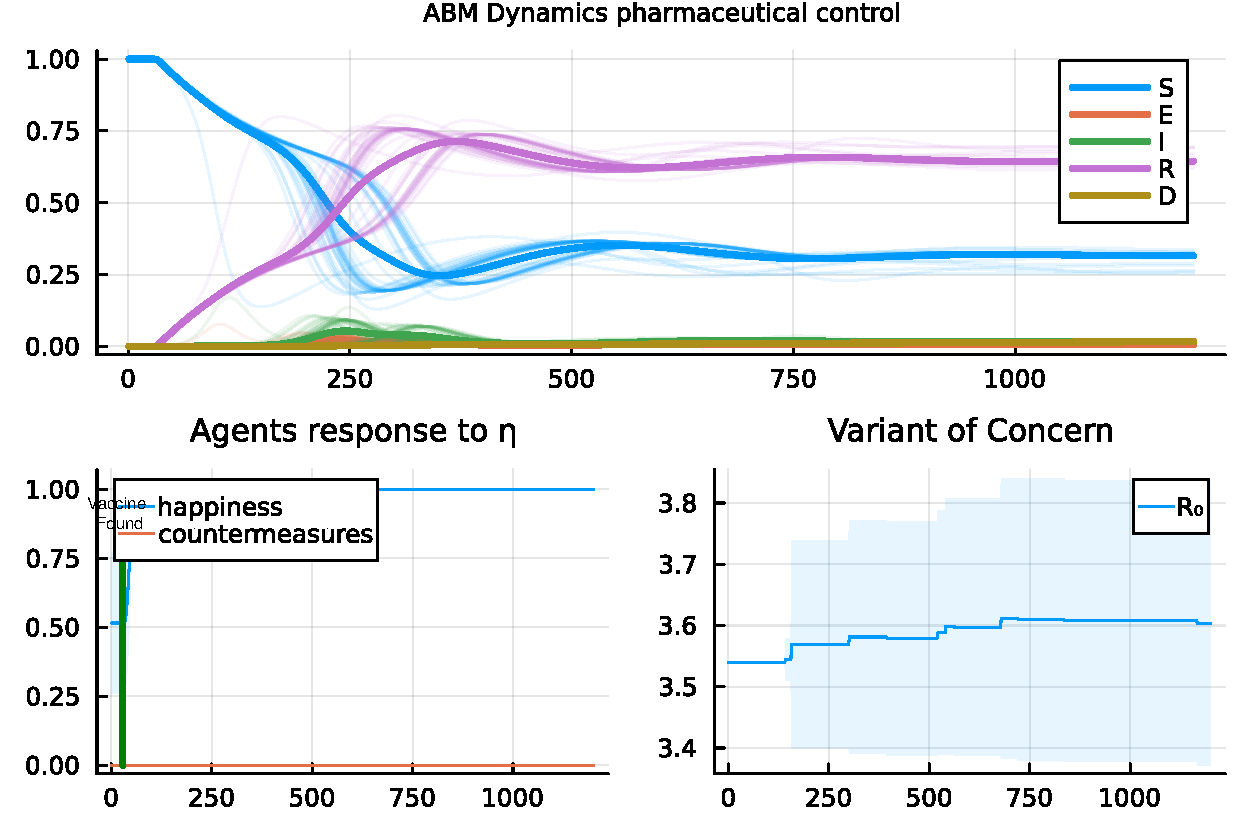
\includegraphics[width=\textwidth]{img/SocialNetworkABM_VACCINE.pdf}
	\captionof{figure}{Grafico cumulativo del modello con intervento del controllore tramite interventi farmaceutici come ad esempio un vaccino}
	\label{fig:abm_vaccine}
\end{minipage}

Il grafico mostra come se disponibili e applicate repentinamente, l'utilizzo di contromisure farmaceutiche permette 
permette di ridurre repentinamente le curve senza andare ad intaccare la curva di happiness in maniera troppo sensibile.
\newpage

\subsection{Intervento farmaceutico e non farmaceutico}
Il seguente grafico \ref{fig:abm_all} mostra l'andamento delle curve del modello
quando questo viene eseguito tramite l'applicazione sia di un intervento di tipo farmaceutico 
come ad esempio l'utillizo di un vaccino, che di contromisure non farmaceutiche.

\begin{minipage}{\linewidth}
	\centering
	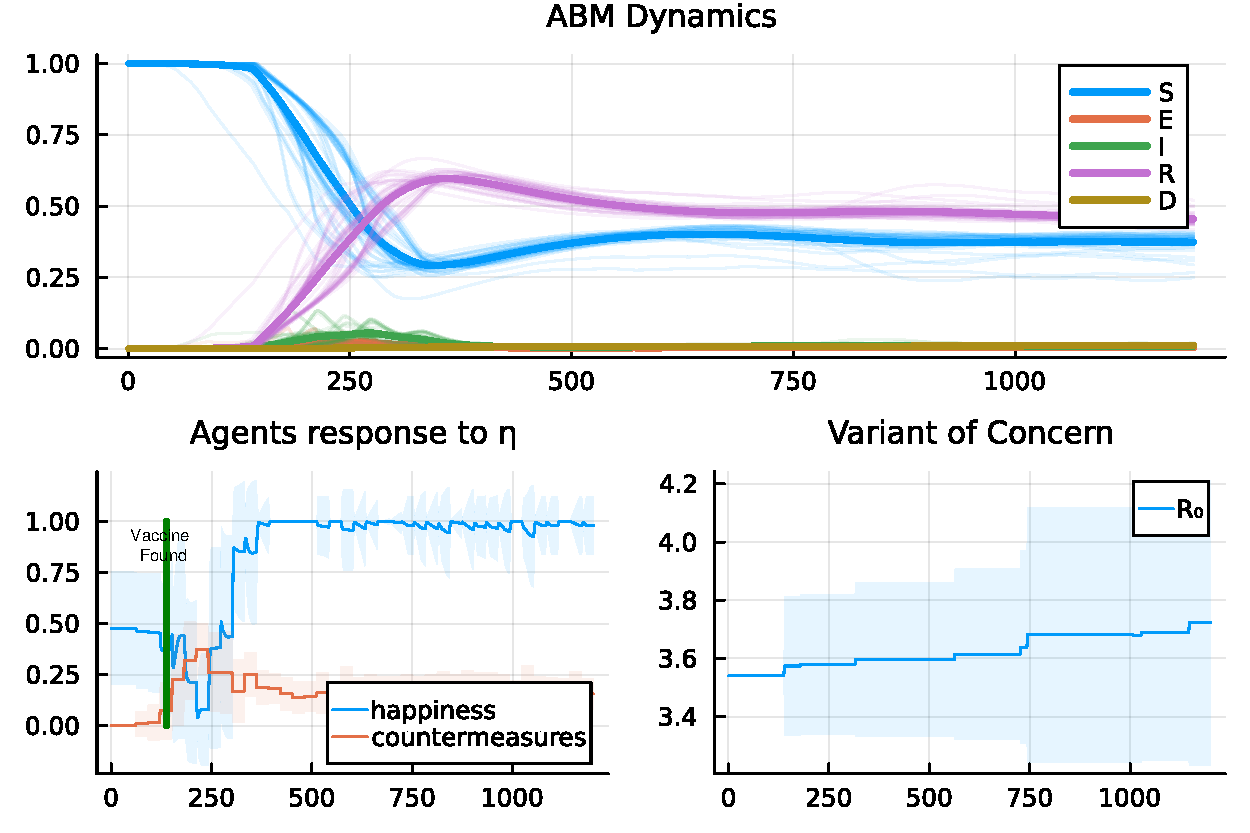
\includegraphics[width=\textwidth]{img/SocialNetworkABM_ALL.pdf}
	\captionof{figure}{Grafico cumulativo del modello con intervento del controllore tramite vaccino e metodi di prevenzione non farmaceutici}
	\label{fig:abm_all}
\end{minipage}

In questo caso viene mostrato l'andamento delle curve tenendo in considerazione l'utilizzo di ogni mezzo
per prevenire e contrastare l'epidemia. L'uitilizzo combinato di mezzi farmaceutici e non permettono 
si appiattire notevolmente la curva di infetti andando a creare velocemente un immunità di gruppo 
che rende la popolazione meno suscettibile alle varianti. Questo inoltre fa si che la \emph{happiness} media
del modello sia generalmente più alta anche quando vengono applicate delle contromisure che vanno ad 
intaccare la felicità della popolazione (ad esempio un lockdown). 

Queste contromisure non farmaceutiche sono in genere meno stringenti e meno prolungate, permettendo quindi
alla popolazione di non avere un calo drastico della happiness generale come in figura \ref{fig:abm_intervent}.
Tuttavia dipendono fortemente da quando le contromisure farmaceutiche (il vaccino) vengono applicate
e con che efficacia questo riesce ad entrare in circolazione. 

Tuttavia questo dimostra come l'utilizzo di un vaccino a priori sia un metodo molto efficace per contrastare
una epidemia, e che ovviamente l'efficacia di questo dipenda molto e soprattutto da quando viene applicato 
alla popolazione. Successivamente si può notare come le misure non farmaceutiche di prevenzione e contrasto
dell'epidemia sono un mezzo efficace per controllare la diffusione dell'infezione, ma queste hanno un costo 
in termini sia di generale qualità della vita, che anche economico, non indifferente come mostrato dai grafici 
precedenti e dall'esperienza diretta che si è avuto con la pandemia da COVID-19. 

\subsection{Analisi di sensitività}
Osservando il modello SEIR definito come segue \ref{fig:ODE_Julia_example} 
si può osservare come quest'ultimo potrebbe essere sensibile al mutamento di specifici 
parametri al suo interno, i quali potrebbero portare il modello ad avere comportamenti 
peculiari e soprattutto imprevisti o inattesi.

Perciò è stato deciso di effettuare un analisi di sensitività del sistema tramite l'utilizzo 
di metodi di libreria offerti dalla suite \emph{SciML.ai}. In questo modo è stato possibile 
osservare a quali parametri il modello fosse più sensibile.

\begin{minipage}{\linewidth}
	\centering
	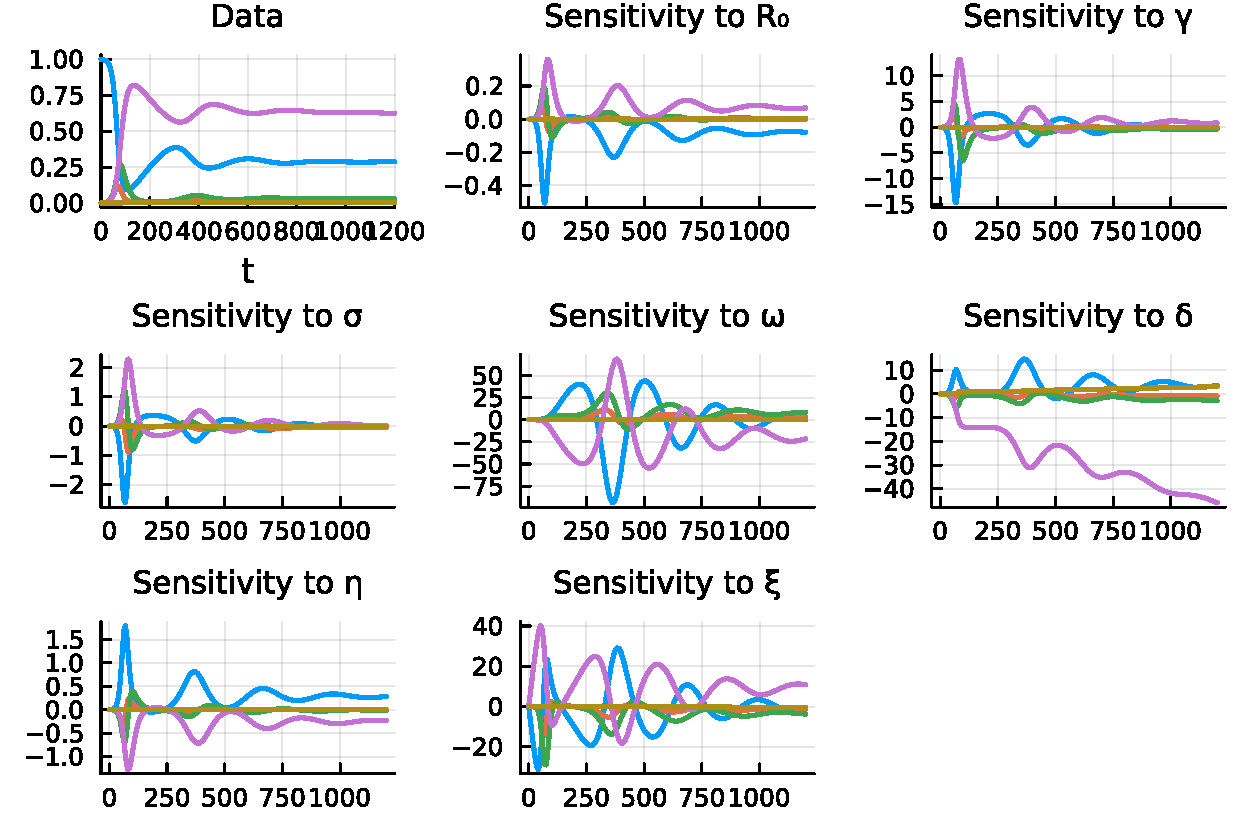
\includegraphics[width=\textwidth]{img/sa.pdf}
	\captionof{figure}{Grafico rappresentante l'analisi di sensitività del modello}
	\label{fig:sens_anal}
\end{minipage}

Come osservato in figura \ref{fig:sens_anal}, il modello ha una sensitività abbastanza 
uniforme per i parametri $R_0, \gamma$ e $\sigma$, il che era atteso in quanto sono tutti 
responsabili dell'avanzamento del contagio. La sensitività ai parametri $\omega$ e $\delta$ 
era comunque attesa, anche se non così accentuata come mostrata in figura. Infine la sensitività 
relativa al parametro $\eta$ responsabile delle contromisure è pressocchè inversa a quella del 
parametro $R_0$ il che è relativamente atteso in quanto è un parametro direttamente collegato 
alle contromisure per la diffusione del contagio. La sensitività al parametro $\xi$ invece ha 
andamento singolare e pare essere legato alla sensitività del parametro $\omega$ seppur in 
modo specchiato. Questo probabilmente perchè essendo i parametri $\omega$ e $\xi$ legati al 
compartimento \textbf{R} del modello, che gestisce gli individui sia guariti che vaccinati, 
il loro comportamento è sensato che sia collegabile.

Successivamente è stata applicato un controllo di sensitività riguardo i parametri 
relativi al modello ad agente in se, tramite l'utilizzo della funzione \textbf{paramscan} offerta
dalla libreria \textbf{Agents.jl}.

è stato scelto un insieme di parametri del modello che vengono modificati all'interno di un range 
definito e in base alle varie configurazioni ottenute si va ad osservare come il comportamento del modello 
può o meno cambiare. I valori che sono stati scelti in quanto idealmente responsabili di un comportamento 
differente se modificati sono i seguenti: 

\begin{minipage}{\linewidth}
	\centering
	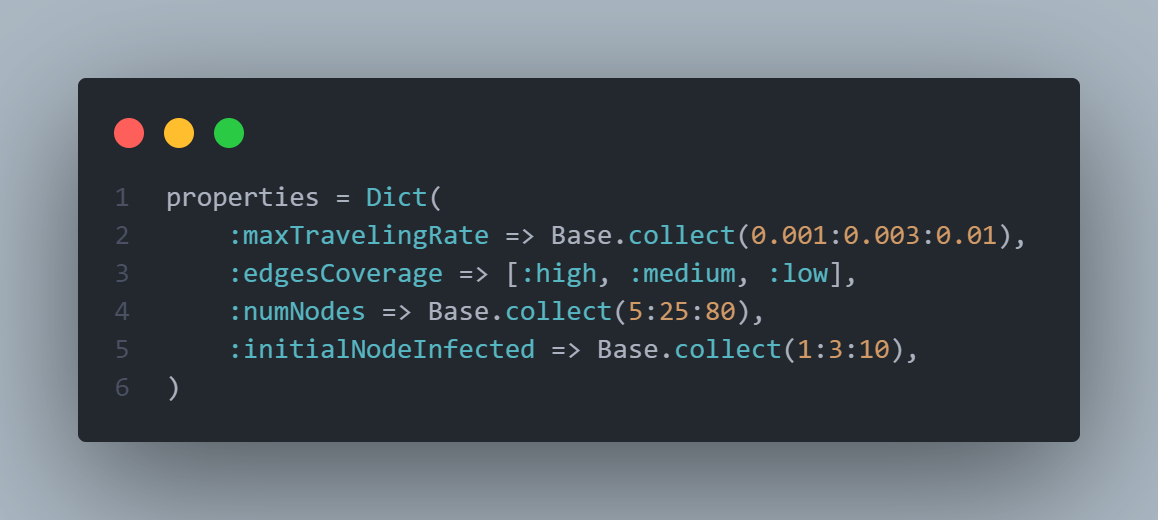
\includegraphics[width=\textwidth]{img/paramscan.png}
	\captionof{figure}{Parametri usati per l'analisi di sensitività del modello ad agente}
	\label{fig:paramscan}
\end{minipage}

Questi parametri sono stati scelti in come possibili parametri con un comportamento latente. I parametri 
relativi al controllore e al vaccino non sono stati inclusi per ovvi motivi, in quanto è stato già dimostrato 
come il loro variare può portare a cambiamenti significativi all'interno della simulazione del modello 
\ref{fig:abm_no_intervent} \ref{fig:abm_intervent} \ref{fig:abm_vaccine} \ref{fig:abm_all}.
\newpage

\subsubsection{Analisi comportamento dato un numero di nodi infetti iniziali variabile}
In questo confronto si nota come il numero di nodi infetti iniziali influenzi principalmente la velocità con cui 
il picco di infetti arriva a compimento. Si nota come nel caso in cui si inizi con un numero di nodi infetti maggiore, 
la curva degli infetti tenderà a essere prona verso l'inizio della linea temporale piuttosto che la fine, arrivando 
al proprio picco prima. Oltre a questo tuttavia non vi sono altri comportamenti degni di nota. Nel complesso è un
comportamento atteso.

\begin{figure}[!hb]
	\centering
	\begin{subfigure}[b]{0.45\textwidth}
		\centering
		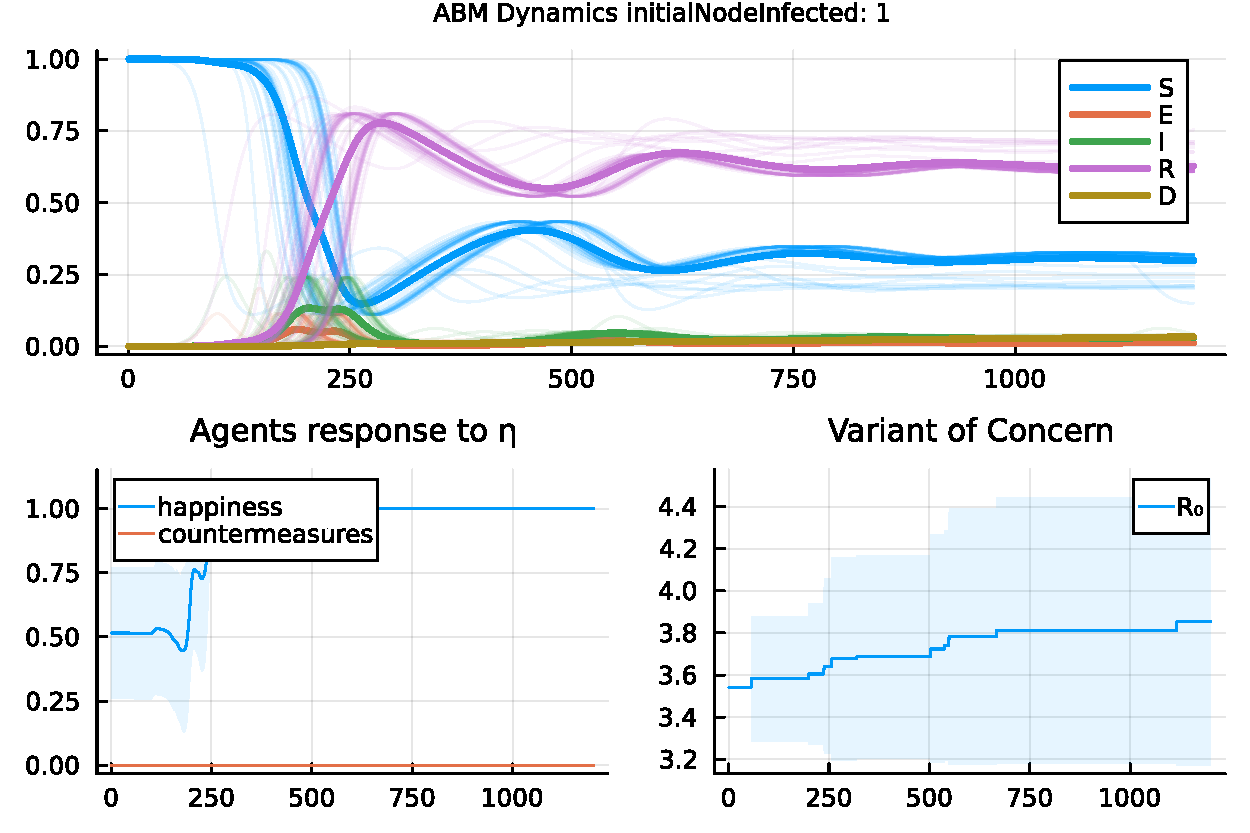
\includegraphics[width=\textwidth]{img/SocialNetworkABM_1_II.pdf}
		\caption{Grafico per la comparazione sul numero di nodi infetti di partenza. Numero nodi infetti iniziali 1}
		\label{fig:comparison_init_node_inf_1}
	\end{subfigure}
	\hfill
	\begin{subfigure}[b]{0.45\textwidth}
		\centering
		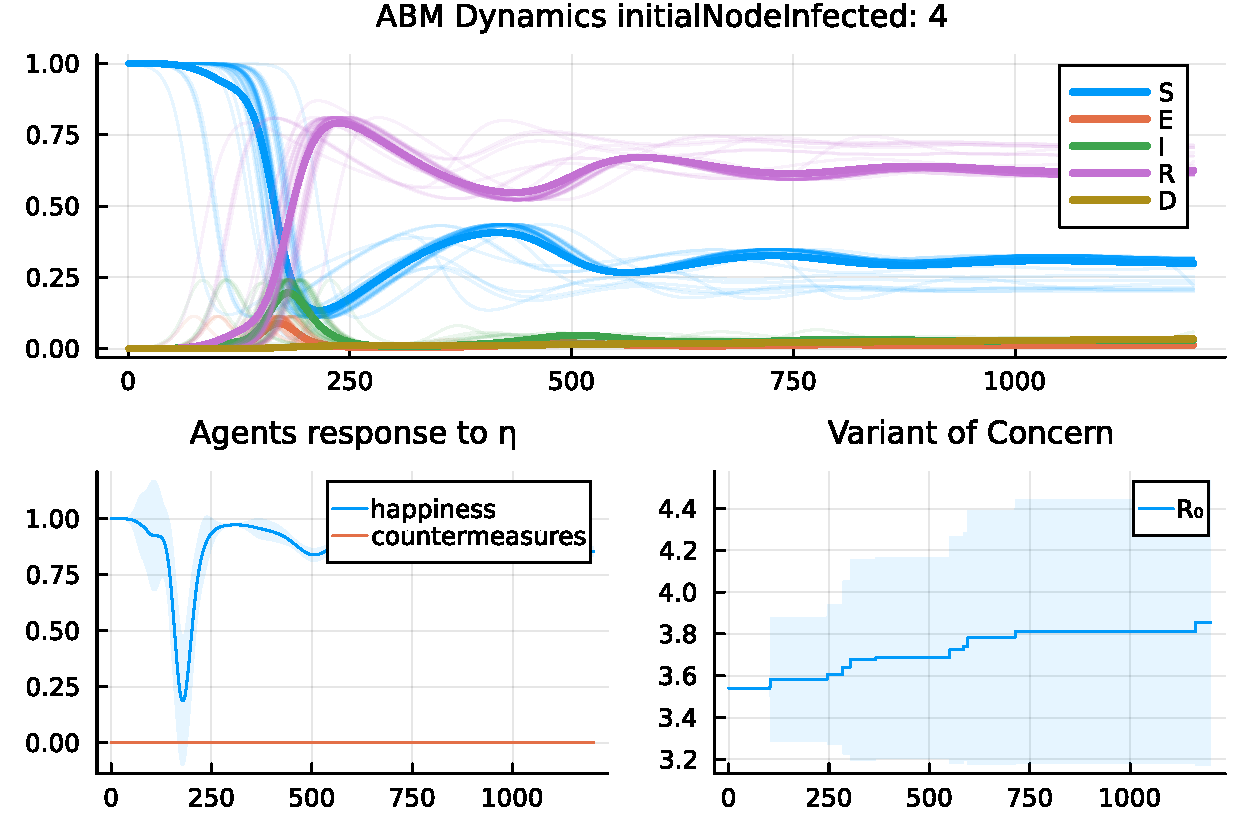
\includegraphics[width=\textwidth]{img/SocialNetworkABM_2_II.pdf}
		\caption{Grafico per la comparazione sul numero di nodi infetti di partenza. Numero nodi infetti iniziali 4}
		\label{fig:comparison_init_node_inf_4}
	\end{subfigure}
	\hfill
	\begin{subfigure}[b]{0.45\textwidth}
		\centering
		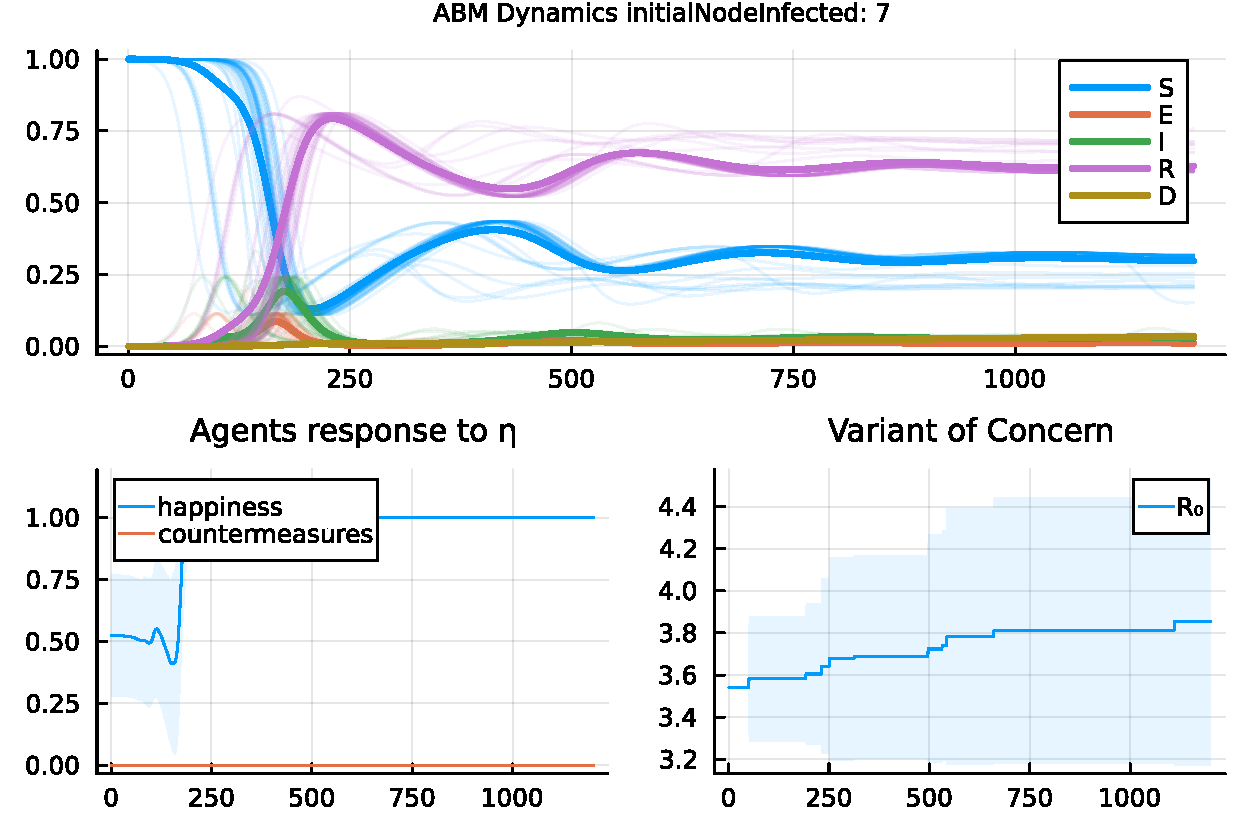
\includegraphics[width=\textwidth]{img/SocialNetworkABM_3_II.pdf}
		\caption{Grafico per la comparazione sul numero di nodi infetti di partenza. Numero nodi infetti iniziali 7}
		\label{fig:comparison_init_node_inf_7}
	\end{subfigure}
	\hfill
	\begin{subfigure}[b]{0.45\textwidth}
		\centering
		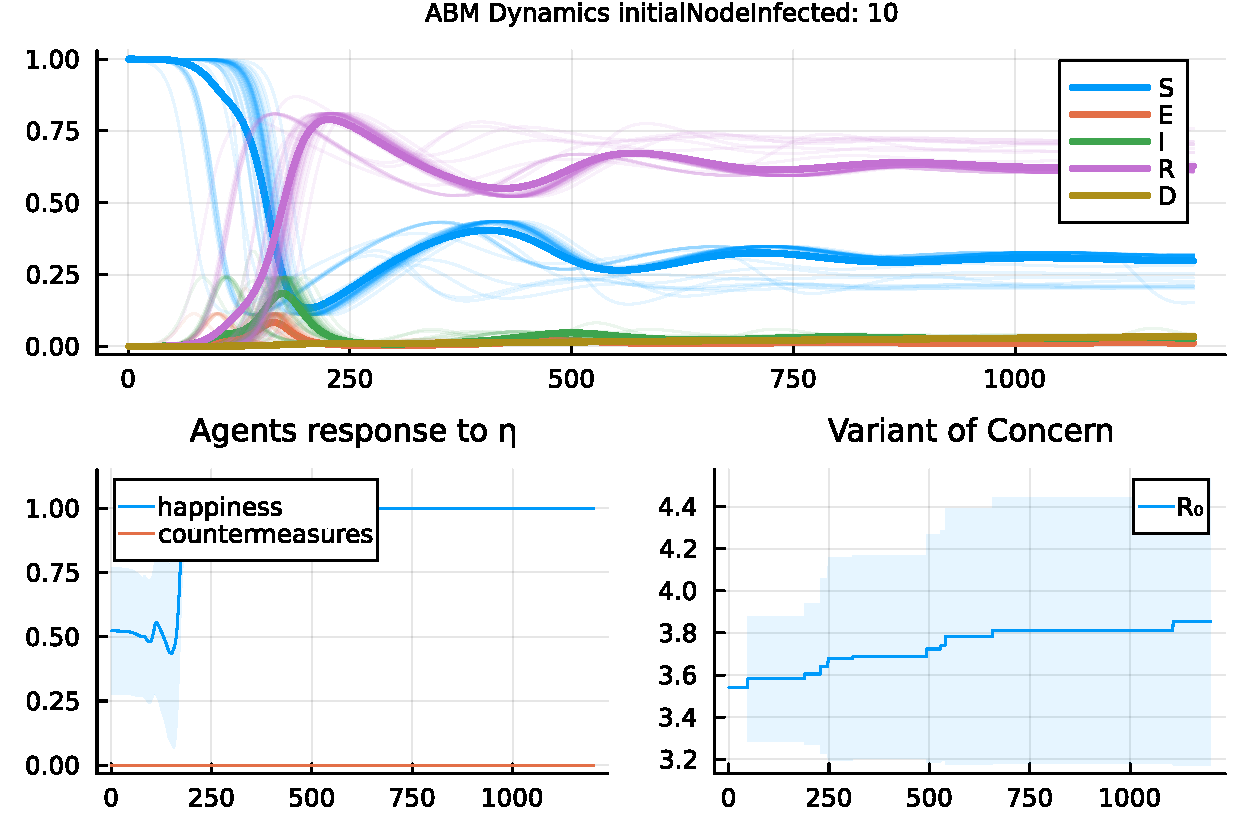
\includegraphics[width=\textwidth]{img/SocialNetworkABM_4_II.pdf}
		\caption{Grafico per la comparazione sul numero di nodi infetti di partenza. Numero nodi infetti iniziali 10}
		\label{fig:comparison_init_node_inf_10}
	\end{subfigure}
\end{figure}
\newpage

\subsubsection{Analisi comportamento dato il valore di migrazione variabile}
Anche in questo caso si può osservare come la curva epidemiologica tenda a raggiungere un valore 
di picco più alto in un periodo di tempo minore nel caso in cui si ha un rateo di migrazione più alto. 
Anche questo comportamento era atteso e non sorprende.

\begin{figure}[!hb]
	\centering
	\begin{subfigure}[b]{0.45\textwidth}
		\centering
		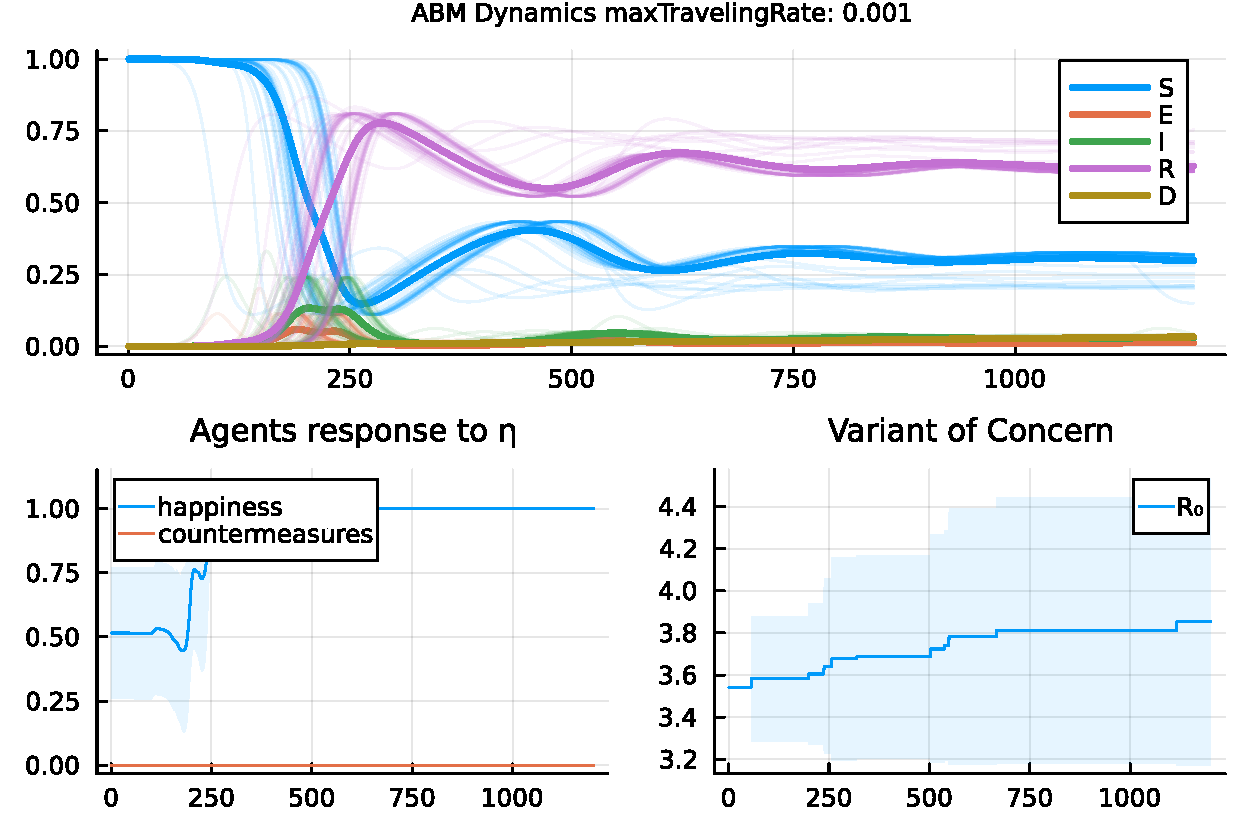
\includegraphics[width=\textwidth]{img/SocialNetworkABM_1_MTR.pdf}
		\caption{Grafico per la comparazione sul valore di migrazione. Valore di 0.001}
		\label{fig:comparison_maxTravelingRate_low}
	\end{subfigure}
	\hfill
	\begin{subfigure}[b]{0.45\textwidth}
		\centering
		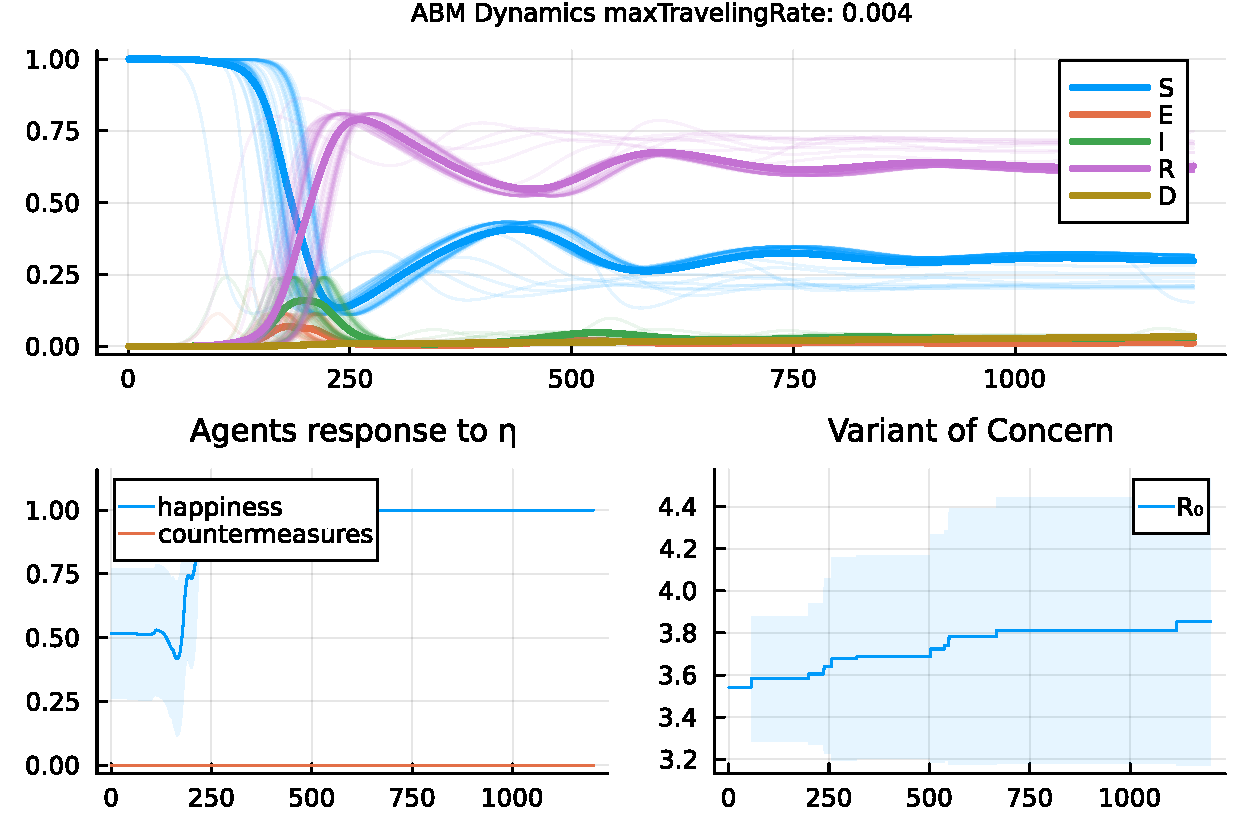
\includegraphics[width=\textwidth]{img/SocialNetworkABM_2_MTR.pdf}
		\caption{Grafico per la comparazione sul valore di migrazione. Valore di 0.004}
		\label{fig:comparison_maxTravelingRate_midl}
	\end{subfigure}
	\hfill
	\begin{subfigure}[b]{0.45\textwidth}
		\centering
		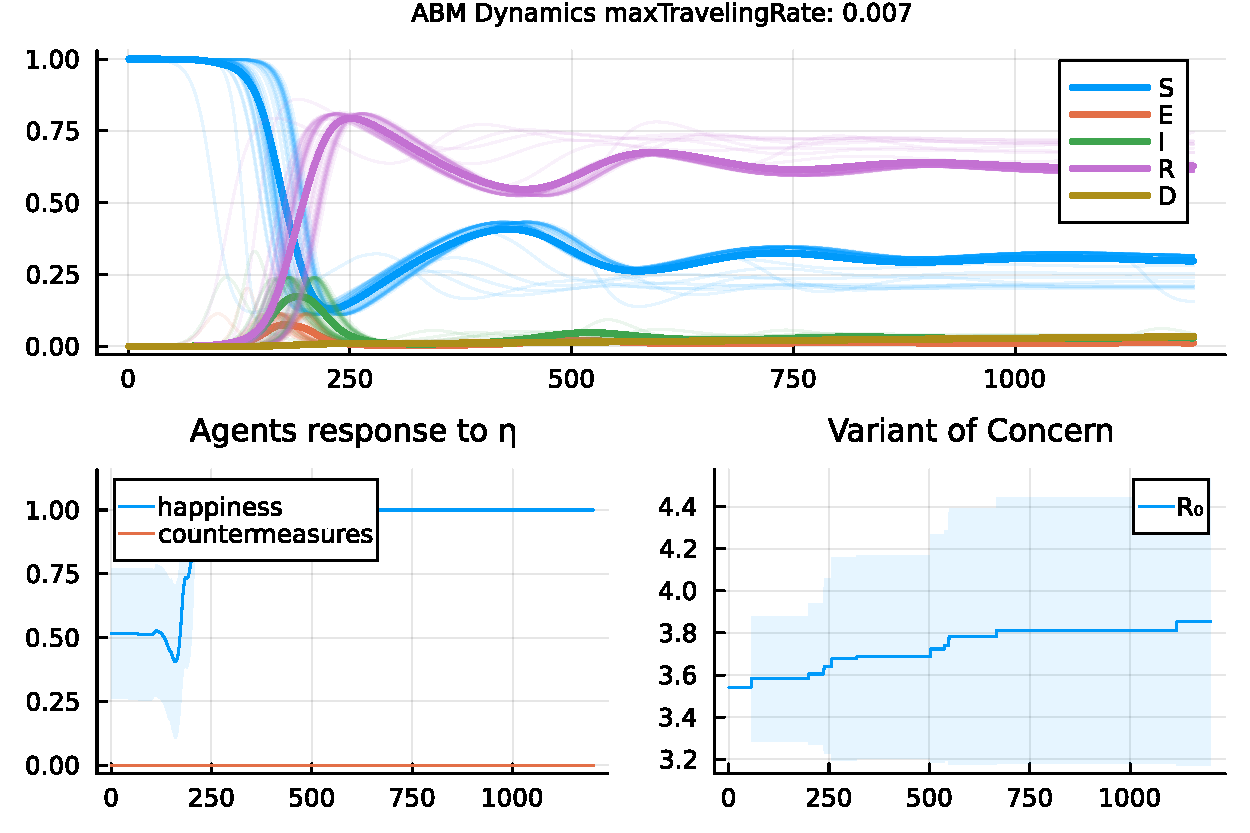
\includegraphics[width=\textwidth]{img/SocialNetworkABM_3_MTR.pdf}
		\caption{Grafico per la comparazione sul valore di migrazione. Valore di 0.007}
		\label{fig:comparison_maxTravelingRate_midh}
	\end{subfigure}
	\hfill
	\begin{subfigure}[b]{0.45\textwidth}
		\centering
		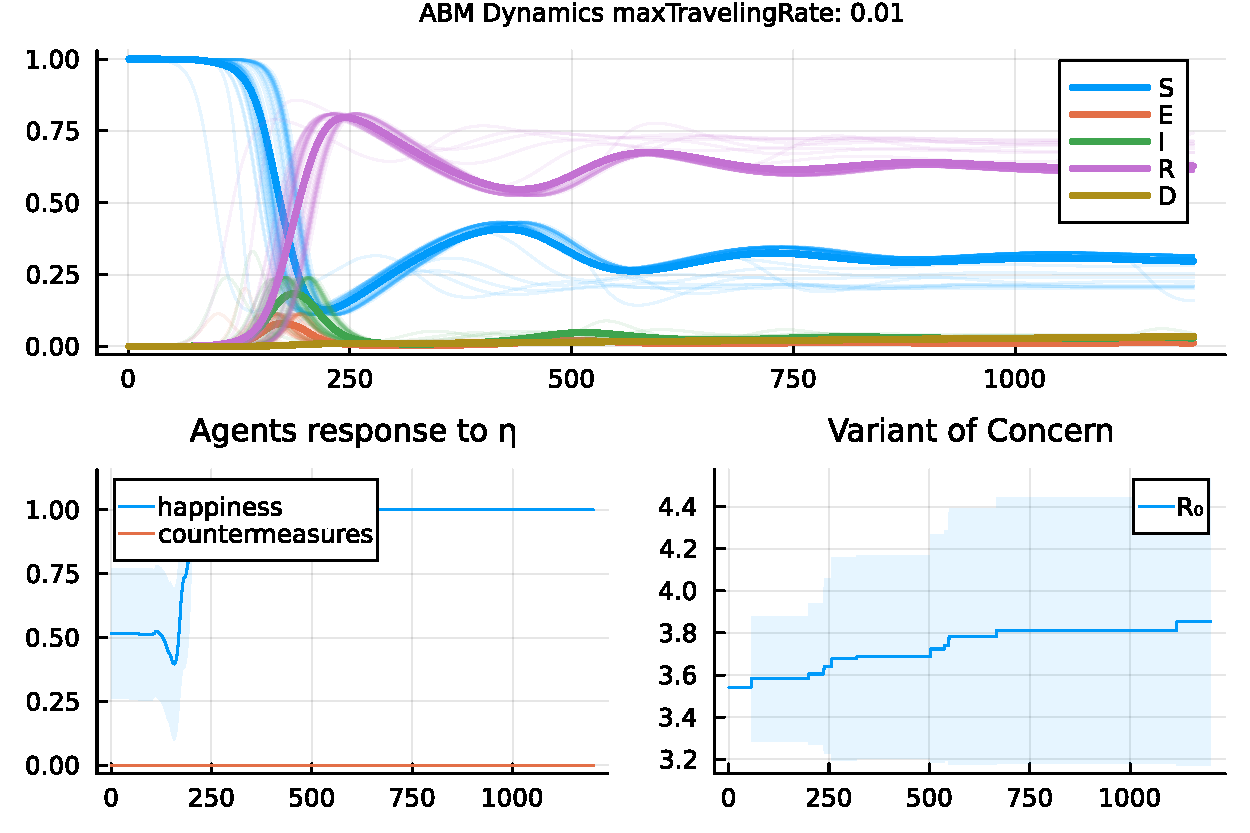
\includegraphics[width=\textwidth]{img/SocialNetworkABM_4_MTR.pdf}
		\caption{Grafico per la comparazione sul valore di migrazione. Valore di 0.01}
		\label{fig:comparison_maxTravelingRate_high}
	\end{subfigure}
\end{figure}

Questo comportamento dipende anche da cosa il parametro \textbf{migrationRate} sta ad indicare. Questo parametro indica il massimo numero 
di individui che possono spostarsi da un nodo di partenza verso un nodo di destinazione. Questo valore viene calcolato quando viene 
creata la matrice di migrazione \ref{fig:migration matrix} e generalmente è un valore \emph{sempre minore} di quello specificato come migrationRate.
\newpage

\subsubsection{Analisi comportamento dato il numero di nodi della rete variabile}
In questo confronto è lapalissiano come il numero di nodi della rete influenzi l'andamento delle curve epidemiologiche. 
I grafici mostrano come in genere un numero di nodi maggiore comporta ad una diffusione più lenta e con picchi meno ripidi
seppur più prolungati nel tempo. Ovviamente questo dipende da molteplici fattori, primo tra tutti la topologia delle connessioni 
del grafo e in secondo luogo dove il primo focolare ha inizio. 

\begin{figure}[!hb]
	\centering
	\begin{subfigure}[b]{0.45\textwidth}
		\centering
		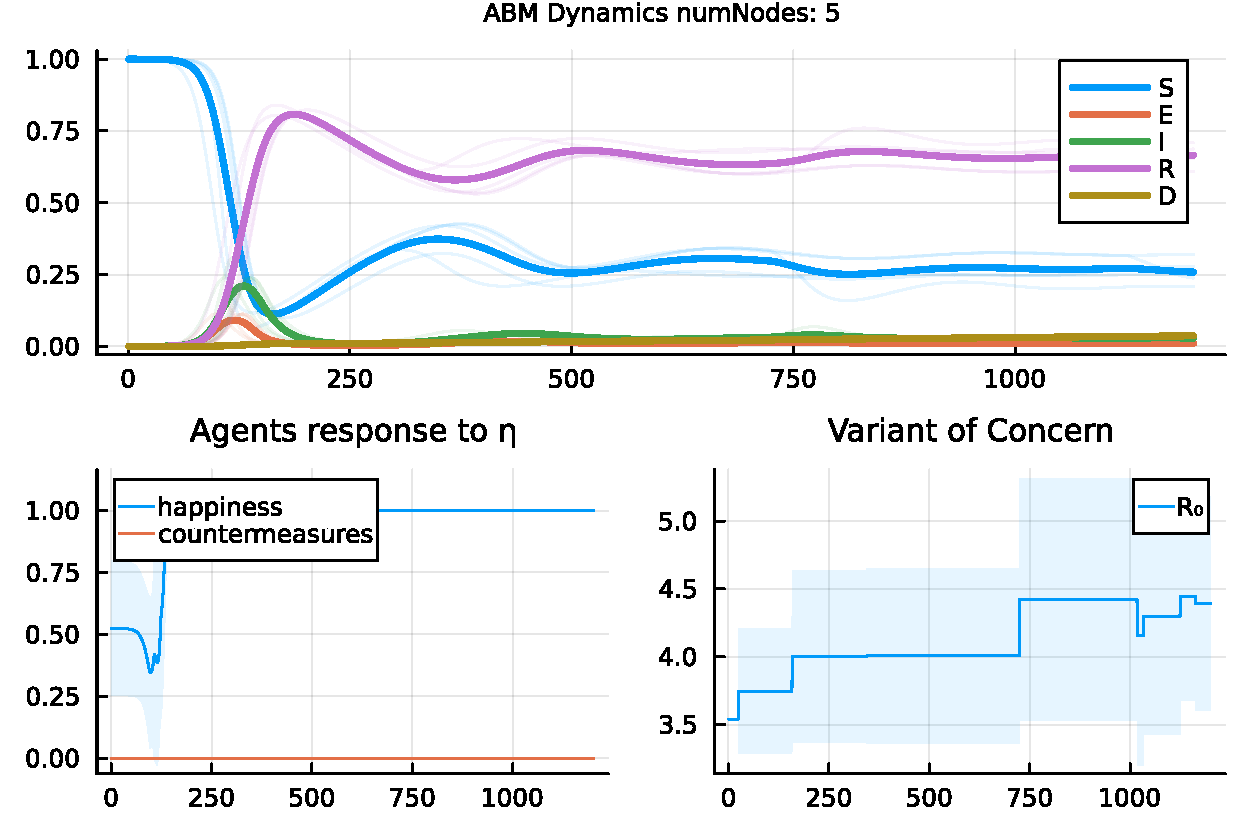
\includegraphics[width=\textwidth]{img/SocialNetworkABM_1_NN.pdf}
		\caption{Grafico per la comparazione sul numero di nodi della rete. Numero nodi 5}
		\label{fig:comparison_numberOfNodes_5}
	\end{subfigure}
	\hfill
	\begin{subfigure}[b]{0.45\textwidth}
		\centering
		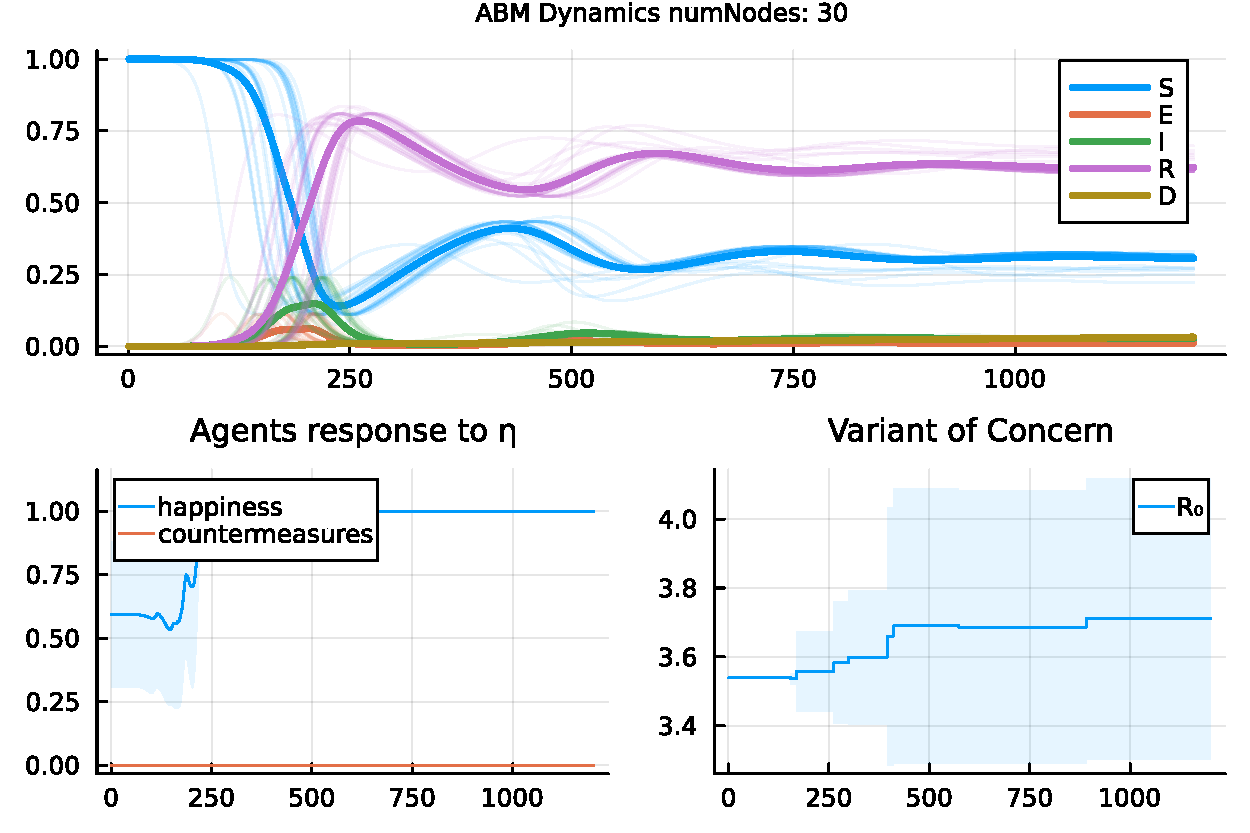
\includegraphics[width=\textwidth]{img/SocialNetworkABM_2_NN.pdf}
		\caption{Grafico per la comparazione sul numero di nodi della rete. Numero nodi 30}
		\label{fig:comparison_numberOfNodes_30}
	\end{subfigure}
	\hfill
	\begin{subfigure}[b]{0.45\textwidth}
		\centering
		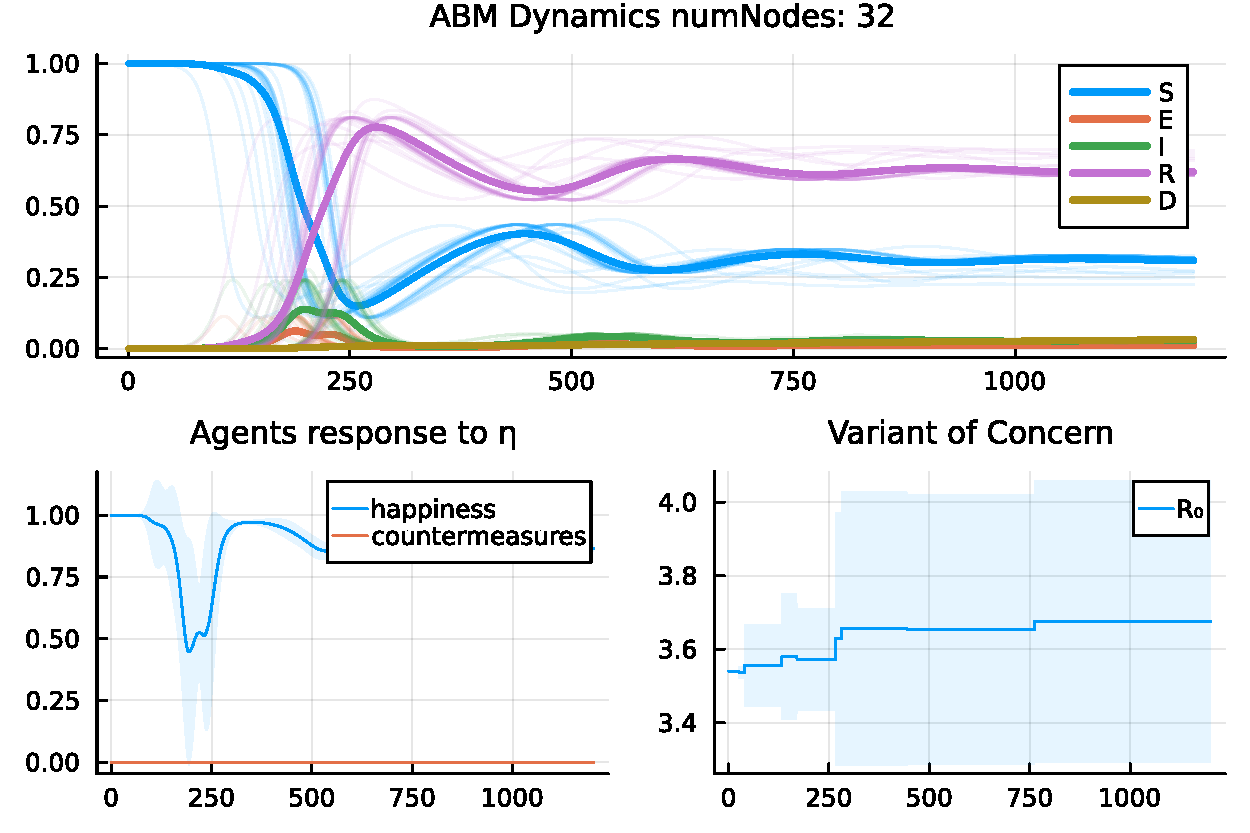
\includegraphics[width=\textwidth]{img/SocialNetworkABM_3_NN.pdf}
		\caption{Grafico per la comparazione sul numero di nodi della rete. Numero nodi 55}
		\label{fig:comparison_numberOfNodes_55}
	\end{subfigure}
	\hfill
	\begin{subfigure}[b]{0.45\textwidth}
		\centering
		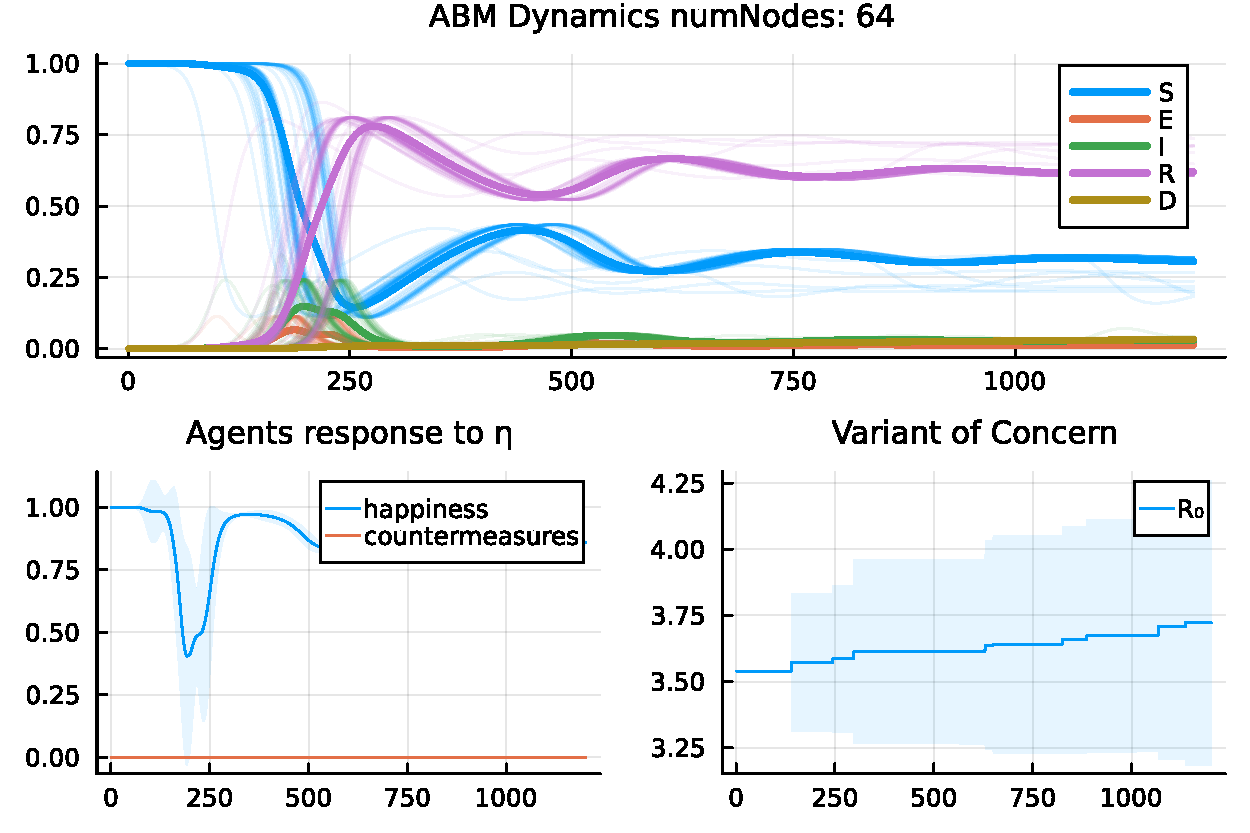
\includegraphics[width=\textwidth]{img/SocialNetworkABM_4_NN.pdf}
		\caption{Grafico per la comparazione sul numero di nodi della rete. Numero nodi 80}
		\label{fig:comparison_numberOfNodes_80}
	\end{subfigure}
\end{figure}
\newpage

\subsubsection{Analisi comportamento data la copertura dei nodi variabile}
In questa figura è osservabile come la copertura della rete, data dal numero di archi che la compongono,
va ad influenzare in maniera sensibile l'andamento della pandemia, soprattutto nel caso in cui la copertura è 
bassa \ref{fig:comparison_lowCoverage}. Tendenzialmente è ipotizzabile che con una bassa copertura, quindi 
con una possibilità più limitata di spostarsi da un nodo all'altro, la diffusione del virus subisce un arresto, 
e questo è osservabile con i dati ottenuti durante la pandemia COVID-19 dove una della prime contromisure applicate 
è stata quella del \textbf{lockdown generalizzato} in cui la capacità di spostamento degli individui 
è calata drasticamente.

\begin{figure}[!hb]
	\centering
	\begin{subfigure}[b]{0.3\textwidth}
		\centering
		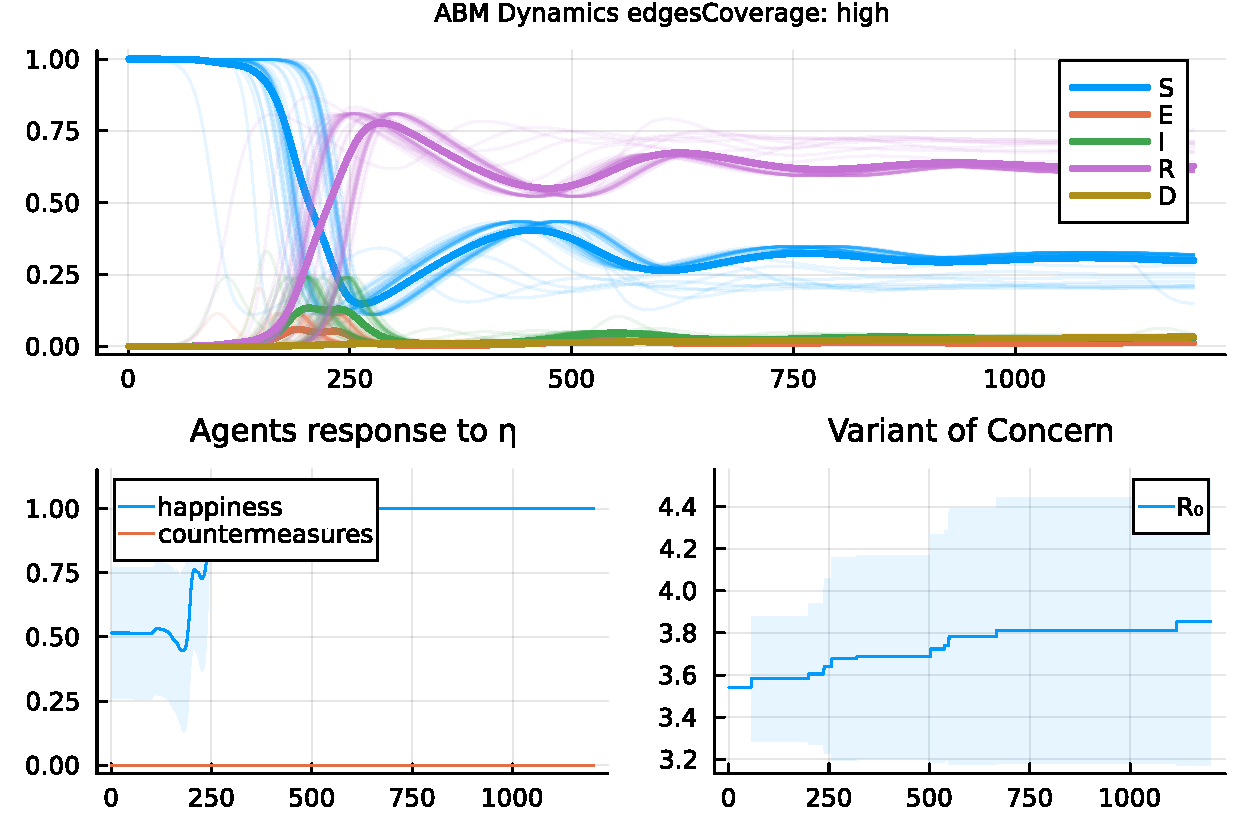
\includegraphics[width=\textwidth]{img/SocialNetworkABM_1_EC.pdf}
		\caption{Grafico per la comparazione sulla copertura della rete. Copertura alta}
		\label{fig:comparison_highCoverage}
	\end{subfigure}
	\hfill
	\begin{subfigure}[b]{0.3\textwidth}
		\centering
		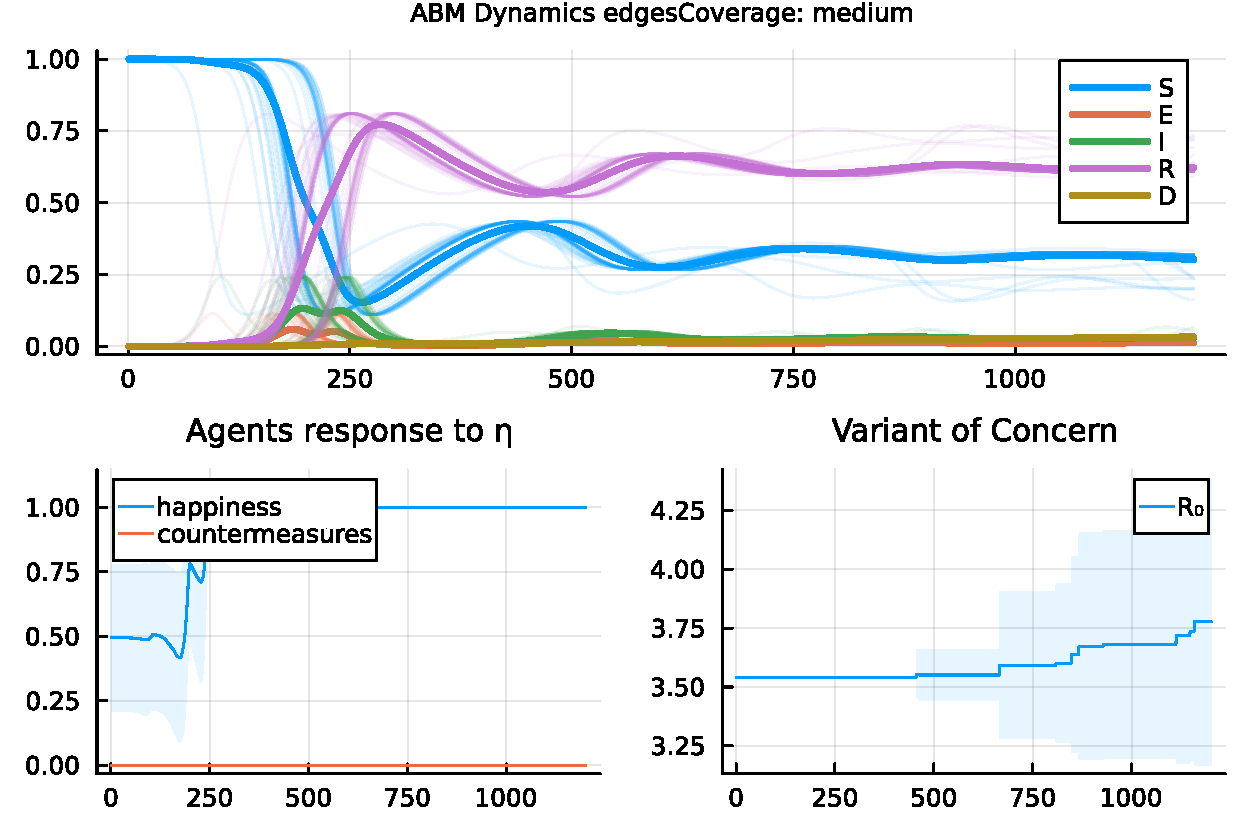
\includegraphics[width=\textwidth]{img/SocialNetworkABM_2_EC.pdf}
		\caption{Grafico per la comparazione sulla copertura della rete. Copertura media}
		\label{fig:comparison_mediumCoverage}
	\end{subfigure}
	\hfill
	\begin{subfigure}[b]{0.3\textwidth}
		\centering
		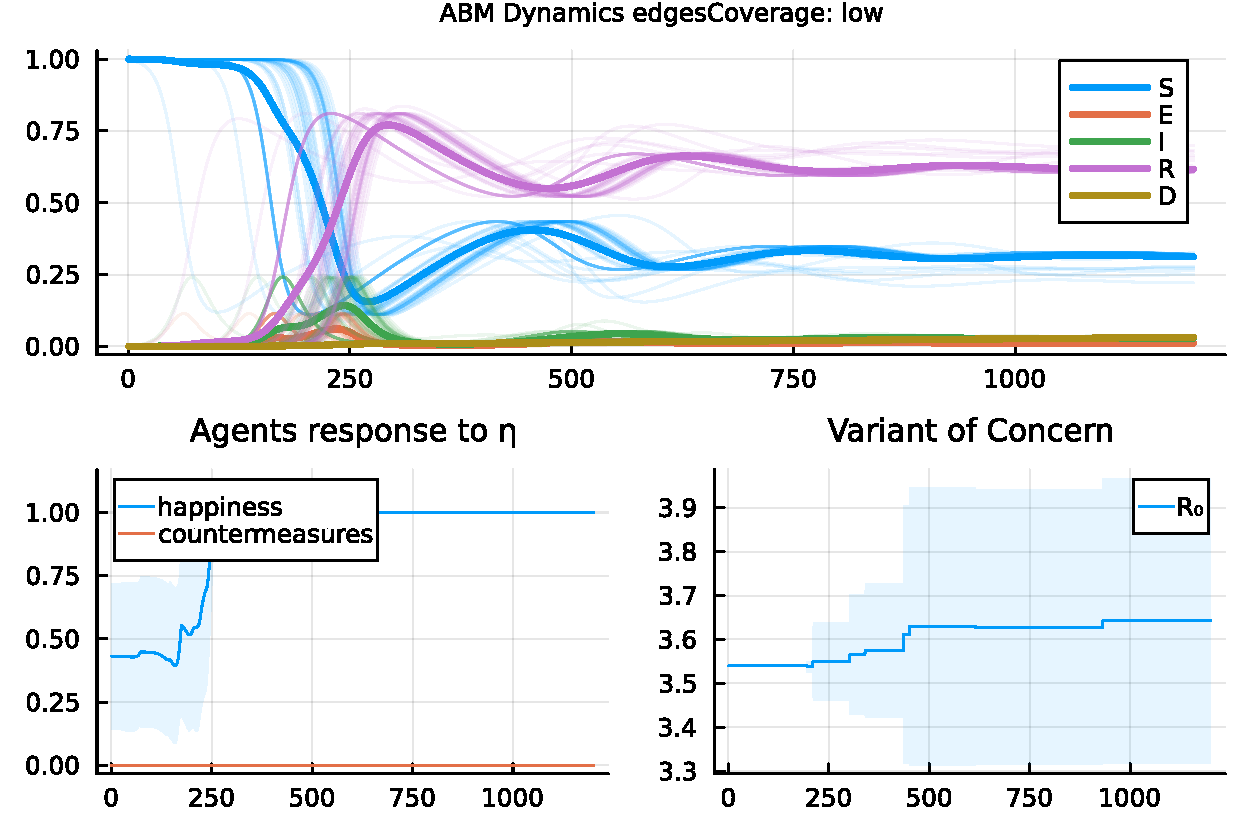
\includegraphics[width=\textwidth]{img/SocialNetworkABM_3_EC.pdf}
		\caption{Grafico per la comparazione sulla copertura della rete. Copertura bassa}
		\label{fig:comparison_lowCoverage}
	\end{subfigure}
\end{figure}

è accurato assumere come, dato il modo con cui viene creata la copertura degli archi, questa 
possa influenzare la diffusione del virus. In particolar modo la diffusione nel caso di alta e media copertura 
è molto simile. Questo è dovuto con molta probabilità al modo in cui viene creata la copertura; modo che 
può essere osservato in figura \ref{fig:graph_coverage}

Ciò nonostante, quello che può essere ulteriormente osservato è il comportamento sempre più "incerto" delle curve 
epidemiologiche al diminuire della copertura del grafo. Discorso similare si può osservare nella comparazione sul numero 
di nodi della rete, in cui le curve epidemiologiche tendono ad assumere un comportamento sempre più incerto all'aumentare dei 
nodi presenti in rete. Anche il numero di \textbf{VOC} pare aumentare con il numero di nodi, questo suggerisce che essendoci 
più individui la possibilità di mutazioni aumenta, così come diminuisce con il diminuire della copertura, stando ad indicare 
come seppur il numero di nodi possa essere elevato, ma se non vi è una possibilità o veicolo di infezione, le mutazioni difficilmente
possono accadere; diminuendo la pericolosità dell'agente patogeno.

\begin{minipage}{\linewidth}
	\centering
	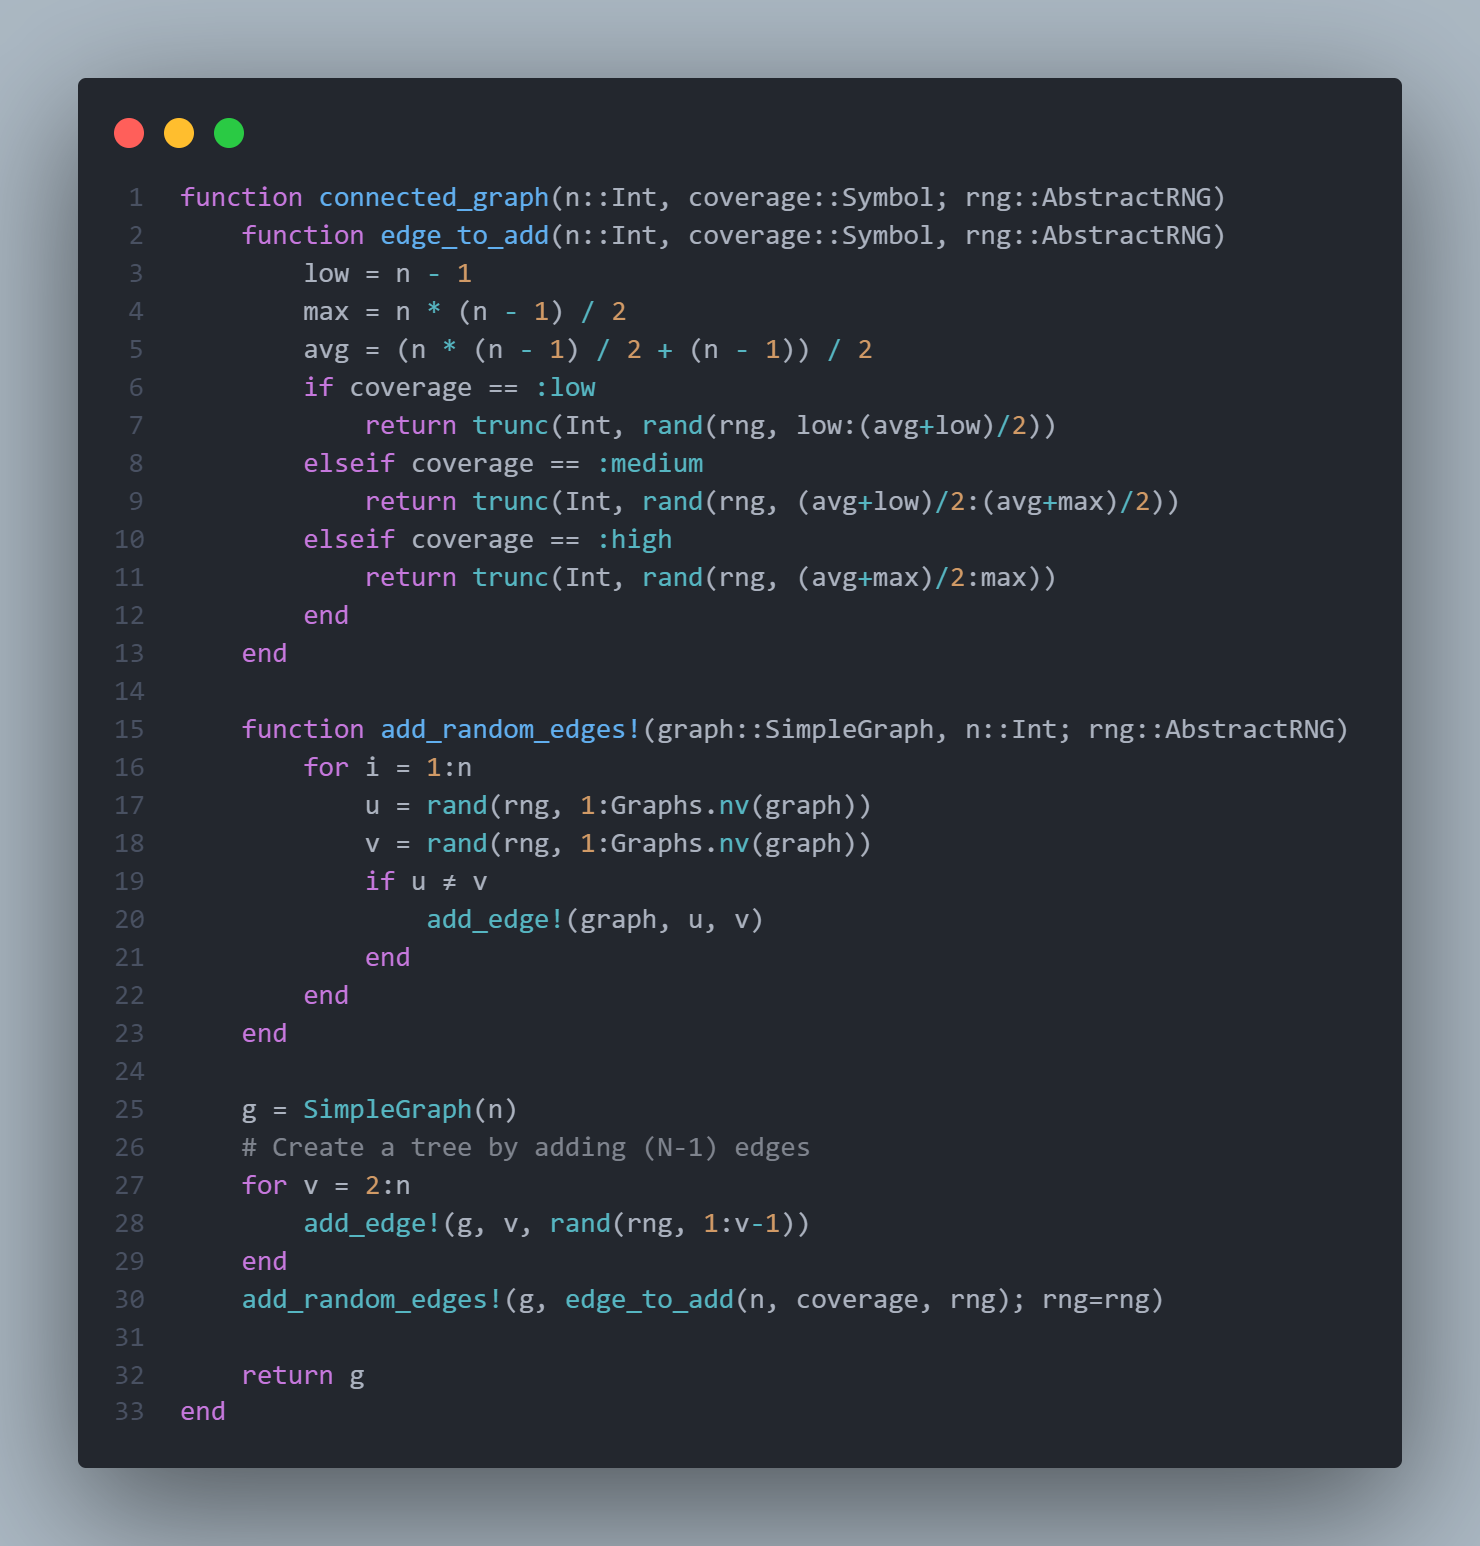
\includegraphics[width=\textwidth]{img/grpah_creation.png}
	\captionof{figure}{Esempio della funzione atta alla creazione di un grafo dato un determinato livello di copertura}
	\label{fig:graph_coverage}
\end{minipage}